\Exercise[number={12}]
Two populations \(w_1\) and \(w_2\) of neurons emit spike trains. The
number \(n\) (integer) of spikes emitted during a certain observation
interval can be described for each of the two populations by a
class-conditioned Poisson type pdf:
\[
    p(n|w_i)=\frac{\lambda_i^n e^{-\lambda_i}}{n!}
\]
where \(\lambda_1\) and \(\lambda_2\) are different for the two
populations. We wanto to build a Bayes classifier that, starting from
the observation of a train of \(n\) spikes, decides from which of the
two populations of neurons it was generated.\\
Determine the boundaries of the decision regions and graphically
describe the result assuming \(\lambda_1>\lambda_2\).

\Answer[number={12}]
Let's write the decision criterion \(z(n)\) by assuming that
\(Pr(w_1)=Pr(w_2)\):
\begin{align*}
    z(n)
    &=\log{\frac{p(n|w_1)}{p(n|w_2)}}+\cancel{\log{\frac{Pr(w_1)}{Pr(w_2)}}}
    =\log{p(n|w_1)}-\log{p(n|w_2)}\\
    &=\log{\frac{\lambda_1^n e^{-\lambda_1}}{n!}}-\log{\frac{\lambda_2^n e^{-\lambda_2}}{n!}}
    =n\log{\lambda_1}-\lambda_1-\cancel{\log{n!}}-n\log{\lambda_2}+\lambda_2+\cancel{\log{n!}}\\
    &=n\log{\frac{\lambda_1}{\lambda_2}}-\lambda_1+\lambda_2
\end{align*}
Hence, the decision boundaries are obtained by setting \(z(n)\) equal to 0:
\begin{align*}
    z(n)=0
    \Longleftrightarrow
    n\log{\frac{\lambda_1}{\lambda_2}}-\lambda_1+\lambda_2=0
    \Rightarrow
    n=\frac{\lambda_1-\lambda_2}{\log{\frac{\lambda_1}{\lambda_2}}}
\end{align*}
Notice that \(\lambda_2<n<\lambda_1\) and that \(n\) is supposed to be an
integer, as the distributions are discrete. All the integers on the
left of \(n=\frac{\lambda_1-\lambda_2}{\log{\frac{\lambda_1}{\lambda_2}}}\)
are classified as class \(w_2\), the integer elements on the right as
class \(w_1\):
\begin{figure}[H]
    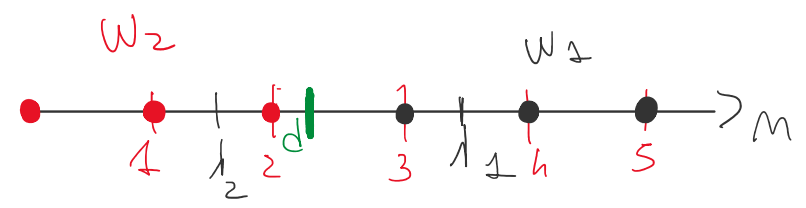
\includegraphics[scale=0.65]{C_12}
    \centering
\end{figure}
If the \(Pr(w_1)\neq{Pr(w_2)}\) assumption is done, then a more complex
expression for the decision boundaries is obtained:
\begin{align*}
    z(n)
    =\dots
    =n\log{\frac{\lambda_1}{\lambda_2}}-\lambda_1+\lambda_2+\log{\frac{Pr(w_1)}{Pr(w_2)}}
\end{align*}
\begin{align*}
    z(n)=0
    \Longleftrightarrow
    n\log{\frac{\lambda_1}{\lambda_2}}-\lambda_1+\lambda_2+\log{\frac{Pr(w_1)}{Pr(w_2)}}=0
    \Rightarrow
    n=\biggl[(\lambda_1-\lambda_2)-\log{\frac{Pr(w_1)}{Pr(w_2)}}\biggr]\frac{1}{\log{\frac{\lambda_1}{\lambda_2}}}
\end{align*}